\usetikzlibrary{shapes.geometric, arrows, positioning}

\def\H{0.9cm}       % Min height for all objects
\def\W{2.15cm}      % Min width of rectangles
\def\Wpill{1.6cm}   % Min width of pills
\def\Wsplit{2.15cm} % Min width for split box (ugly solution)
\def\distV{1.4cm}   % Vertical distance between objects
\def\distH{0.6cm}   % Horizontal distance between objects


% Style
%\tikzstyle{every node} = [font=\tiny]
\tikzstyle{every node} = [font=\scriptsize]
\tikzstyle{every path} = [thick]
\tikzstyle{arrow} = [thick,->,>=stealth]

% Objects
\tikzstyle{startstop} = [rectangle, minimum width=\Wpill, minimum height=\H, text centered, draw=black, rounded corners=\H/2]
\tikzstyle{process}   = [rectangle, minimum width=\W, minimum height=\H, text centered, draw=black]
\tikzstyle{decision}  = [diamond,   minimum width=\H, minimum height=\H, text centered, draw=black]


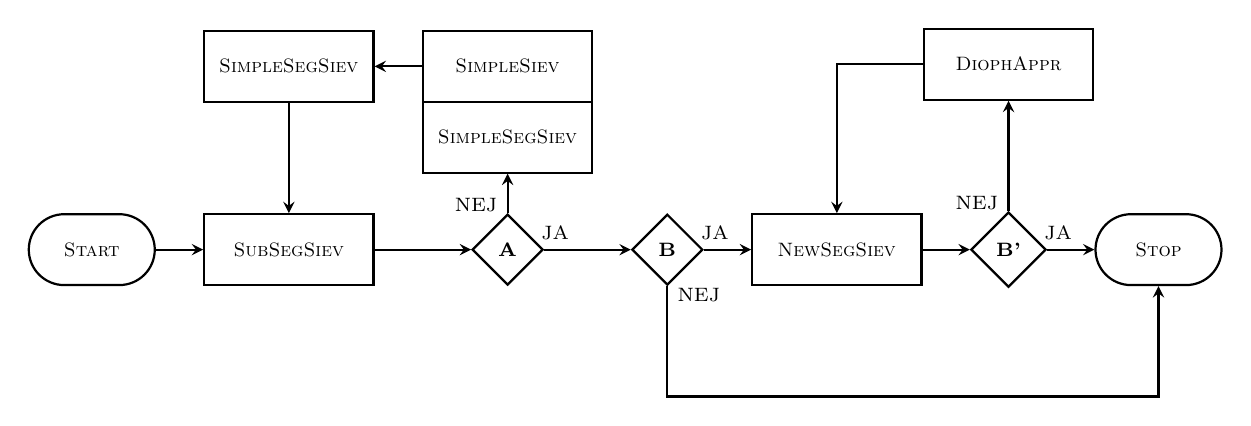
\begin{tikzpicture}
% Objects
    % Start
    \node (start) [startstop]                       {\textsc{Start}};
    % First loop
    \node (sub)   [process,  right=\distH of start] {\textsc{SubSegSiev}};
    \node (sim2)  [process,  above=\distV of sub]   {\textsc{SimpleSegSiev}};

    \node (sim1)  [process,  right=\distH of sim2, minimum width=\Wsplit]  {\textsc{SimpleSiev}};
    \node (sim0)  [process,  below=-\pgflinewidth of sim1, minimum width=\Wsplit]  {\textsc{SimpleSegSiev}};
    \node (A)     [decision, below=\distV of sim1]  {\textbf{A}};
    % Middle
    \node (B0)    [decision, right=\distH + 0.5cm of A]     {\textbf{B}};
    % Second loop
    \node (new)   [process,  right=\distH of B0]    {\textsc{NewSegSiev}};
    \node (B1)    [decision, right=\distH of new]   {\textbf{B'}};
    \node (dio)   [process,  above=\distV of B1]    {\textsc{DiophAppr}};
    % Stop
    \node (stop)  [startstop,right=\distH of B1]    {\textsc{Stop}};

% Arrows
    % Start to first loop
    \draw [arrow] (start) -- (sub);
    % First loop
    \draw [arrow] (sub)   -- (A);
    \draw [arrow] (A)     -- (sim0);
    \draw [arrow] (sim1)  -- (sim2);
    \draw [arrow] (sim2)  -- (sub);
    % Middle
    \draw [arrow] (A)     -- (B0);
    \draw [arrow] (B0)    -- (new);
    \draw [arrow] (B0)    |- ([yshift=-\distV]B0.south) -| (stop);
    % Second loop
    \draw [arrow] (new)   -- (B1);
    \draw [arrow] (B1)    -- (dio);
    \draw [arrow] (dio)   -| (new);
    \draw [arrow] (B1)    -- (stop);

% Decision texts
    \node[above=3pt of A,  anchor=east]  {NEJ};
    \node[right=4pt of A,  anchor=south] {JA};
    \node[below=3pt of B0, anchor=west]  {NEJ};
    \node[right=4pt of B0, anchor=south] {JA};
    \node[above=3pt of B1, anchor=east]  {NEJ};
    \node[right=4pt of B1, anchor=south] {JA};
\end{tikzpicture}
\vspace{0.5cm}